\section{Utente Non Autenticato}
%1)who is he? add a reference/description to this actor in the general description's list of roles
%2) È corretto
   %dal punto di vista della sicurezza che un utente non ancora identificato
   %nell’applicazione possa creare contenuti (Company)?
%3) Give a more expressive name to paragraphs

Di seguito vengono elencati i \glossaryItem{casi d'uso} per l'utente non autenticato.

\subsection{Casi d'uso}

\subsubsection{Operazioni dell'utente non autenticato}
  
    \begin{figure}[H]
      \begin{center}
        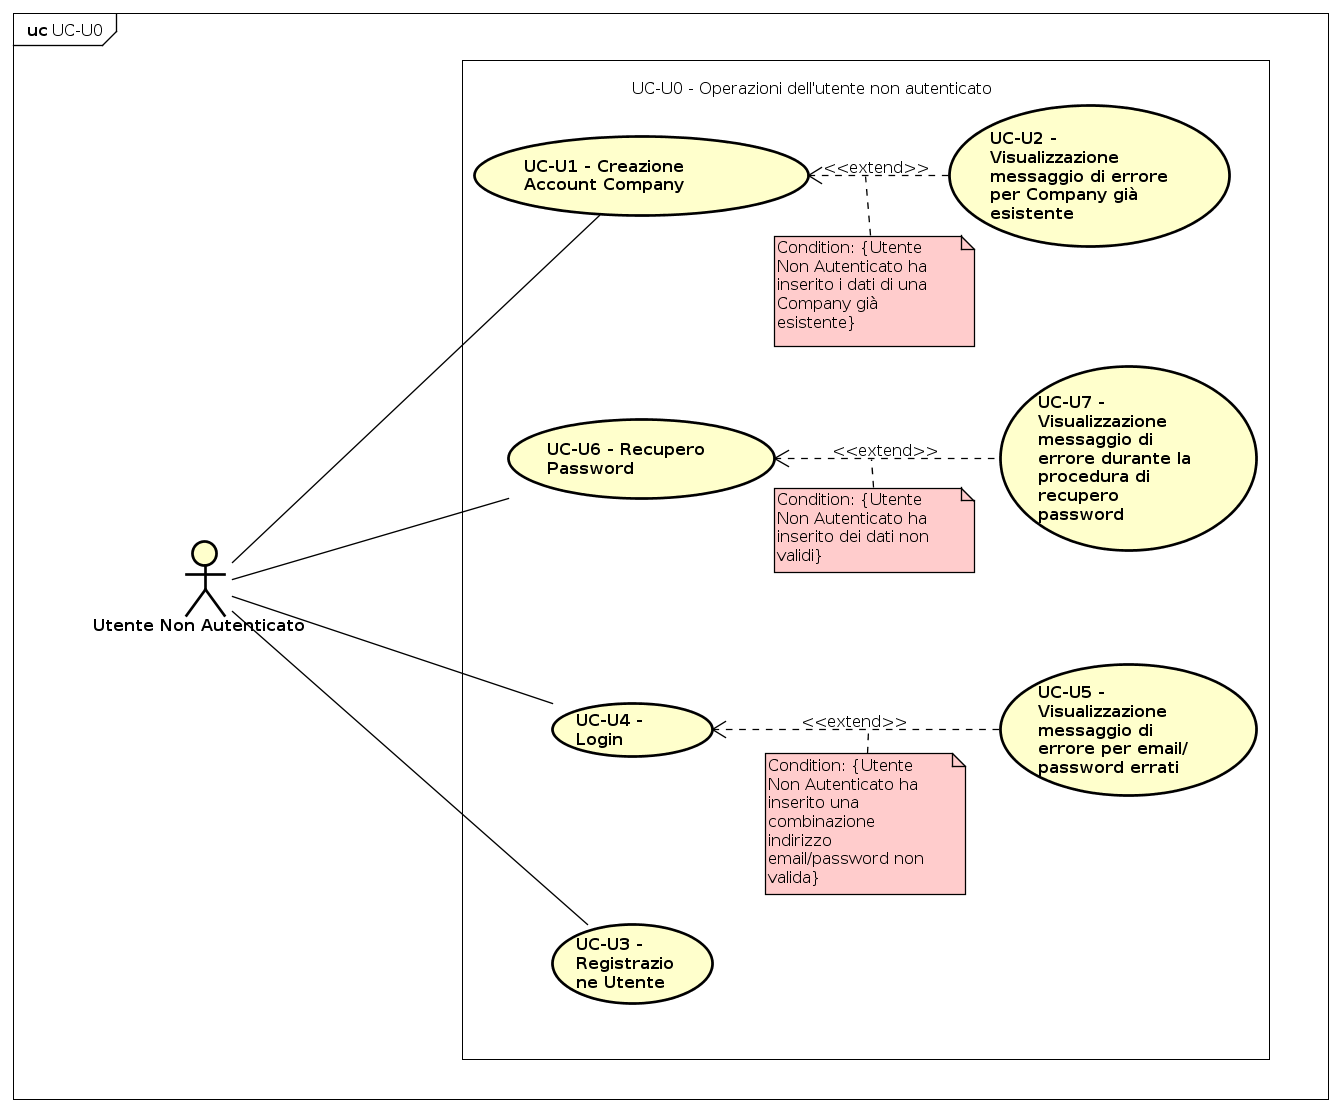
\includegraphics[width=12cm]{res/img/UCUtenti/UCUtenteNA/UC-U0.png}
      \caption{UC-U0 - Operazioni dell'utente non autenticato}
      \end{center} 
    \end{figure}    
    
    %Tabella 
    \begin{center}
      \bgroup
      \def\arraystretch{1.8}     
      \begin{longtable}{  p{3.5cm} | p{8cm} } 
        
        \hline
        \multicolumn{2}{ | c | }{ \cellcolor[gray]{0.9} \textbf{UC-U0 - Operazioni dell'utente non autenticato}} \\ 
        \hline
        
        \textbf{Attori Primari} & Utente non autenticato \\ 
        \textbf{Scopo e Descrizione} & L’utente non autenticato può creare un nuovo account per la propria \glossaryItem{Company} e registrarsi a \glossaryItem{MaaS}, oppure effettuare la registrazione dopo aver ricevuto un invito. Può effettuare il login e il recupero della propria password. \\ 
        
        \textbf{Precondizioni}  & L’applicazione è funzionante e pronta all’utilizzo.
        
        Il sistema mostra all’utente non autenticato la pagina principale fornendo le funzionalità di autenticazione, registrazione e recupero password. \\ 
        
        \textbf{Postcondizioni} & L'applicazione ha eseguito le richieste dell'utente. \\ 
        \textbf{Scenario principale} & 1. L'utente non autenticato crea un account per la propria \glossaryItem{Company} e si registra a \glossaryItem{MaaS} come \glossaryItem{Owner}. (UC-U1)
        
2. L'utente non autenticato riceve un invito per registrarsi a \glossaryItem{MaaS}. (UC-U3)

3. L'utente non autenticato in possesso di un account  effettua il login. (UC-U4)

4. L'utente non autenticato può richiedere il recupero della password. (UC-U6) \\
        \textbf{Estensioni} & 1. L'utente non autenticato visualizza un messaggio di errore dovuto all'inserimento di dati di una \glossaryItem{Company} già esistente. (UC-U2)
        
2. L'utente non autenticato visualizza un messaggio d'errore durante il login dovuto all'inserimento di un indirizzo email/password non corretti. (UC-U5)

3. L'utente non autenticato visualizza un messaggio d'errore durante la \glossaryItem{procedura} di recupero password. (UC-U7)  \\
      \end{longtable}
      \egroup
    \end{center} 
    
\subsubsection{Creazione account di una Company}

    \begin{figure}[H]
      \begin{center}
        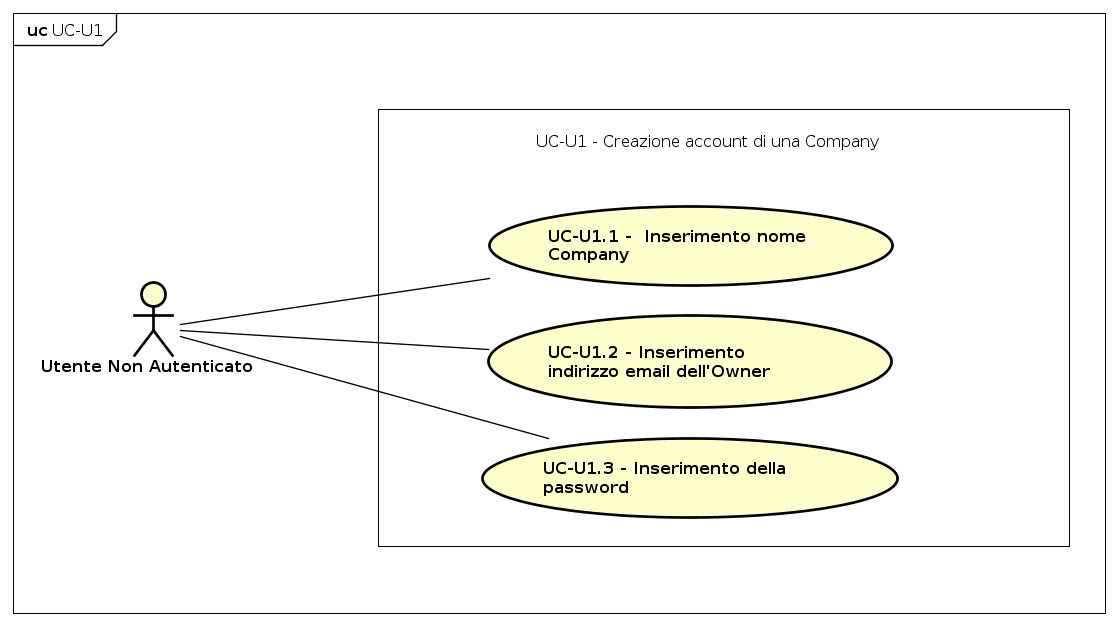
\includegraphics[width=12cm]{res/img/UCUtenti/UCUtenteNA/UC-U1-Creazione Account Azienda/UC-U1.png}
      \caption{UC-U1 - Creazione account di una \glossaryItem{Company}}
      \end{center} 
    \end{figure}    
    
    %Tabella 
    \begin{center}
      \bgroup
      \def\arraystretch{1.8}     
      \begin{longtable}{  p{3.5cm} | p{8cm} } 
        
        \hline
        \multicolumn{2}{ | c | }{ \cellcolor[gray]{0.9} \textbf{UC-U1 - Creazione account di una \glossaryItem{Company}}} \\ 
        \hline
        
        \textbf{Attori Primari} & Utente non autenticato \\ 
        \textbf{Scopo e Descrizione} & L'utente non autenticato può creare un account per la propria \glossaryItem{Company}, inserendo i seguenti dati: nome della \glossaryItem{Company}, indirizzo email dell'\glossaryItem{Owner} e una password. \\ 
        
        \textbf{Precondizioni}  & L’applicazione è funzionante e pronta all’utilizzo.
        
Il sistema presenta all'utente la pagina di registrazione per una \glossaryItem{Company}. \\ 
        
        \textbf{Postcondizioni} & Una \glossaryItem{Company} è stata registrata presso \glossaryItem{MaaS} e l'utente non autenticato ne è divenuto l'\glossaryItem{Owner}. \\ 
        \textbf{Scenario principale} & 1. L'utente non autenticato inserisce il nome della propria \glossaryItem{Company}. (UC-U1.1)
        
2. L'utente non autenticato inserisce il proprio indirizzo email. (UC-U1.2)

3. L'utente non autenticato inserisce una password e la \glossaryItem{Company} viene registrata. (UC-U1.3) \\
      \end{longtable}
      \egroup
    \end{center} 
    
\subsubsection{Inserimento nome Company}    
    
    %Tabella 
    \begin{center}
      \bgroup
      \def\arraystretch{1.8}     
      \begin{longtable}{  p{3.5cm} | p{8cm} } 
        
        \hline
        \multicolumn{2}{ | c | }{ \cellcolor[gray]{0.9} \textbf{UC-U1.1 - Inserimento nome \glossaryItem{Company}}} \\ 
        \hline
        
        \textbf{Attori Primari} & Utente non autenticato \\ 
        \textbf{Scopo e Descrizione} & L'utente non autenticato inserisce il nome della \glossaryItem{Company} durante la \glossaryItem{procedura} di creazione dell'account. \\ 
        
        \textbf{Precondizioni}  & 
L'utente non autenticato ha visualizzato la pagina per la creazione dell'account di una \glossaryItem{Company}. \\ 
        
        \textbf{Postcondizioni} & Il campo testo \`e stato compilato con il contenuto richiesto. \\ 
        \textbf{Scenario principale} & 1. L'utente non autenticato inserisce il nome della \glossaryItem{Company} durante la \glossaryItem{procedura} di creazione dell'account. (UC-1.1) \\
      \end{longtable}
      \egroup
    \end{center} 


\subsubsection{Inserimento indirizzo email dell'Owner}   
    
    %Tabella 
    \begin{center}
      \bgroup
      \def\arraystretch{1.8}     
      \begin{longtable}{  p{3.5cm} | p{8cm} } 
        
        \hline
        \multicolumn{2}{ | c | }{ \cellcolor[gray]{0.9} \textbf{UC-U1.2 - Inserimento indirizzo email dell'\glossaryItem{Owner}}} \\ 
        \hline
        
        \textbf{Attori Primari} & Utente non autenticato \\ 
        \textbf{Scopo e Descrizione} & L'utente non autenticato inserisce il proprio indirizzo email durante la \glossaryItem{procedura} di creazione dell'account della \glossaryItem{Company}. \\ 
        
        \textbf{Precondizioni}  & L'utente non autenticato ha visualizzato la pagina per la creazione dell'account
        di una \glossaryItem{Company}.  \\ 
        
        \textbf{Postcondizioni} & Il campo testo \`e stato compilato con il contenuto richiesto. \\
         \textbf{Scenario principale} & 1. L'utente non autenticato inserisce il proprio indirizzo email durante la \glossaryItem{procedura} di creazione dell'account della \glossaryItem{Company}. (UC-1.2)\\ 
      \end{longtable}
      \egroup
    \end{center} 
    
\subsubsection{Inserimento della password} 
    
    %Tabella 
    \begin{center}
      \bgroup
      \def\arraystretch{1.8}     
      \begin{longtable}{  p{3.5cm} | p{8cm} } 
        
        \hline
        \multicolumn{2}{ | c | }{ \cellcolor[gray]{0.9} \textbf{UC-U1.3 - Inserimento della password}} \\ 
        \hline
        
        \textbf{Attori Primari} & Utente non autenticato \\ 
        \textbf{Scopo e Descrizione} & L'utente non autenticato inserisce la password associata all'account della propria \glossaryItem{Company}. \\ 
        
        \textbf{Precondizioni}  & L'utente non autenticato ha visualizzato la pagina per la registrazione della \glossaryItem{Company}. \\ 
        
        \textbf{Postcondizioni} & L'utente non autenticato ha inserito una password associata all'account della \glossaryItem{Company}. \\ 
        \textbf{Scenario principale} & 1. L'utente non autenticato inserisce una password associata all'account della \glossaryItem{Company}. (UC-1.3)\\
      \end{longtable}
      \egroup
    \end{center}

\subsubsection{Messaggio d’errore per Company già esistente}   
    
    %Tabella 
    \begin{center}
      \bgroup
      \def\arraystretch{1.8}     
      \begin{longtable}{  p{3.5cm} | p{8cm} } 
        
        \hline
        \multicolumn{2}{ | c | }{ \cellcolor[gray]{0.9} \textbf{UC-U2 - Messaggio d’errore per \glossaryItem{Company} già esistente}} \\ 
        \hline
        
        \textbf{Attori Primari} & Utente non autenticato \\ 
        \textbf{Scopo e Descrizione} & L'utente non autenticato visualizza un messaggio d'errore dovuto all'inserimento di dati di una \glossaryItem{Company} già registrata. \\ 
        
        \textbf{Precondizioni}  & L'utente ha inserito i dati di una \glossaryItem{Company} già registrata. \\ 
        
        \textbf{Postcondizioni} & L'utente ha visualizzato il messaggio di errore. \\ 
        \textbf{Scenario principale} & 1. L'utente visualizza il messaggio di errore. \\
      \end{longtable}
      \egroup
    \end{center} 

\subsubsection{Registrazione Utente}

    \begin{figure}[H]
      \begin{center}
        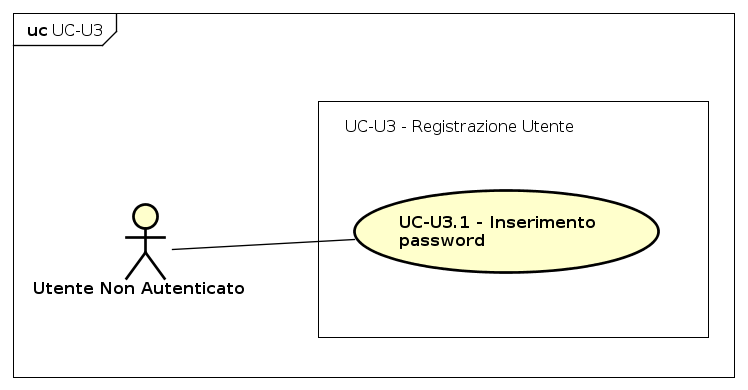
\includegraphics[width=12cm]{res/img/UCUtenti/UCUtenteNA/UC-U3-Registrazione Utente/UC-U3.png}
      \caption{UC-U3 - Registrazione Utente}
      \end{center} 
    \end{figure}    
    
    %Tabella 
    \begin{center}
      %1) L'esito dice che il \glossaryItem{processo} di registrazione non è chiaro
      %2) È corretto che l’utente debba inserire unicamente la password e debba farlo una volta sola?
      \bgroup
      \def\arraystretch{1.8}     
      \begin{longtable}{  p{3.5cm} | p{8cm} } 
        
        \hline
        \multicolumn{2}{ | c | }{ \cellcolor[gray]{0.9} \textbf{UC-U3 - Registrazione Utente}} \\ 
        \hline
        
        \textbf{Attori Primari} & Utente non autenticato \\ 
        \textbf{Scopo e Descrizione} & L'utente non autenticato può registrarsi su \glossaryItem{MaaS} con un invito precedentemente ricevuto dall'\glossaryItem{Owner} della \glossaryItem{Company} di appartenenza o da un suo delegato. \\ 
        
        \textbf{Precondizioni}  & L'utente ha ricevuto un invito dall'\glossaryItem{Owner} o da un suo delegato. \\ 
        
        \textbf{Postcondizioni} & L'utente non autenticato ha creato un account valido e può effettuare il login. \\ 
        \textbf{Scenario principale} & 1. L'utente inserisce la propria password. (UC-U3.1) \\
      \end{longtable}
      \egroup
    \end{center} 

\subsubsection{Login}

    \begin{figure}[H]
      \begin{center}
        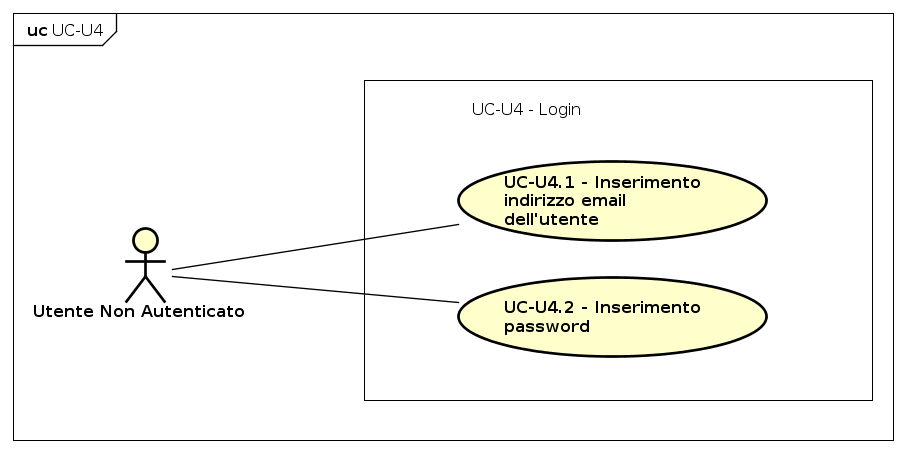
\includegraphics[width=12cm]{res/img/UCUtenti/UCUtenteNA/UC-U4-Login/UC-U4.png}
      \caption{UC-U4 - Login}
      \end{center} 
    \end{figure}    
    
    %Tabella 
    \begin{center}
      \bgroup
      \def\arraystretch{1.8}     
      \begin{longtable}{  p{3.5cm} | p{8cm} } 
        
        \hline
        \multicolumn{2}{ | c | }{ \cellcolor[gray]{0.9} \textbf{UC-U4 - Login}} \\ 
        \hline
        
        \textbf{Attori Primari} & Utente non autenticato \\ 
        \textbf{Scopo e Descrizione} & L'utente non autenticato può effettuare il login all'applicazione. \\ 
        
        \textbf{Precondizioni}  & L'utente non autenticato è in possesso di un account valido. \\ 
        
        \textbf{Postcondizioni} & L'utente non autenticato viene autenticato e ha accesso alle funzionalità dell'applicazione concesse in base al ruolo espresso nel suo account. \\ 
        \textbf{Scenario principale} & 1. L'utente non autenticato inserisce il proprio indirizzo email (UC-U4.1)
        
2. L'utente non autenticato inserisce la password (UC-U4.2) \\
      \end{longtable}
      \egroup
    \end{center} 
    
\subsubsection{Inserimento indirizzo email dell'utente}  
   
    %Tabella 
    \begin{center}
      \bgroup
      \def\arraystretch{1.8}     
      \begin{longtable}{  p{3.5cm} | p{8cm} } 
        
        \hline
        \multicolumn{2}{ | c | }{ \cellcolor[gray]{0.9} \textbf{UC-U4.1 - Inserimento indirizzo email dell'utente}} \\ 
        \hline
        
        \textbf{Attori Primari} & Utente non autenticato \\ 
        \textbf{Scopo e Descrizione} & L'utente non autenticato inserisce il proprio indirizzo email. \\ 
        
        \textbf{Precondizioni}  & L'utente non autenticato è in possesso di un account valido. \\ 
        

        \textbf{Postcondizioni} & Il campo testo \`e stato compilato con il contenuto richiesto. \\
         \textbf{Scenario principale} & 1. L'utente non autenticato inserisce il proprio indirizzo email.
      \end{longtable}
      \egroup
    \end{center} 

\subsubsection{Inserimento password utente}
    
    %Tabella 
    \begin{center}
      \bgroup
      \def\arraystretch{1.8}     
      \begin{longtable}{  p{3.5cm} | p{8cm} } 
        
        \hline
        \multicolumn{2}{ | c | }{ \cellcolor[gray]{0.9} \textbf{UC-U4.2 - Inserimento password utente}} \\ 
        \hline
        
        \textbf{Attori Primari} & Utente non autenticato \\ 
        \textbf{Scopo e Descrizione} & L'utente non autenticato inserisce la password associata al proprio account. \\ 
        
        \textbf{Precondizioni}  & L'utente non autenticato è in possesso di un account valido. \\ 
        
        \textbf{Postcondizioni} & Il campo testo \`e stato compilato con il contenuto richiesto. \\

         \textbf{Scenario principale} & 1. L'utente non autenticato inserisce la password associata al proprio account.
      \end{longtable}
      \egroup
    \end{center}
    
\subsubsection{Messaggio d’errore per email/password non corretti}   
    
    %Tabella 
    \begin{center}
      \bgroup
      \def\arraystretch{1.8}     
      \begin{longtable}{  p{3.5cm} | p{8cm} } 
        
        \hline
        \multicolumn{2}{ | c | }{ \cellcolor[gray]{0.9} \textbf{UC-U5 - Messaggio d’errore per email/password non corretti}} \\ 
        \hline
        
        \textbf{Attori Primari} & Utente non autenticato \\ 
        \textbf{Scopo e Descrizione} & L'utente non autenticato visualizza un messaggio d'errore dovuto all'inserimento di un indirizzo email o di una password non corretti durante la \glossaryItem{procedura} di Login. \\ 
        
        \textbf{Precondizioni}  & L'utente ha inserito un indirizzo email o una password non corretti. \\ 
        
        \textbf{Postcondizioni} & L'utente ha visualizzato il messaggio di errore. \\ 
        \textbf{Scenario principale} & 1. L'utente visualizza il messaggio di errore. \\
      \end{longtable}
      \egroup
    \end{center}    

\subsubsection{Recupero password}

    \begin{figure}[H]
      \begin{center}
        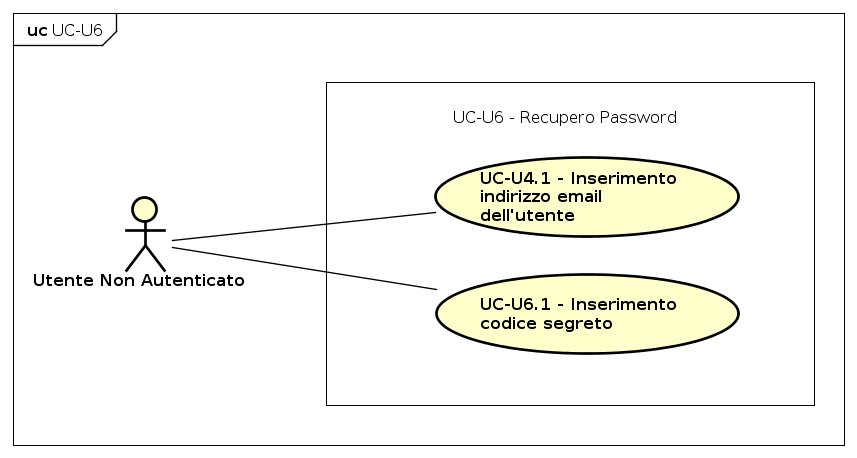
\includegraphics[width=12cm]{res/img/UCUtenti/UCUtenteNA/UC-U6-Recupero Password/UC-U6.png}
      \caption{UC-U6 - Recupero password}
      \end{center} 
    \end{figure}    
    
    %Tabella 
    \begin{center}
      \bgroup
      \def\arraystretch{1.8}     
      \begin{longtable}{  p{3.5cm} | p{8cm} } 
        
        \hline
        \multicolumn{2}{ | c | }{ \cellcolor[gray]{0.9} \textbf{UC-U6 - Recupero password}} \\ 
        \hline
        
        \textbf{Attori Primari} & Utente non autenticato \\ 

        \textbf{Scopo e Descrizione} & L'utente non autenticato effettua la \glossaryItem{procedura} per il recupero della password, inserendo il proprio indirizzo email e il codice segreto che gli verrà inviato dal sistema. \\ 
        
        \textbf{Precondizioni}  & L'utente possiede un account all'interno dell'applicazione. \\ 
        
        \textbf{Postcondizioni} & L'utente non autenticato ha ottenuto una nuova password per accedere all'applicazione. \\ 
        \textbf{Scenario principale} & 1. L'utente non autenticato inserisce il proprio indirizzo email. (UC-U4.1)
        
2. L'utente non autenticato inserisce il codice segreto ricevuto. (UC-U6.1) \\
      \end{longtable}
      \egroup
    \end{center} 

\subsubsection{Inserimento codice segreto} 
    
    %Tabella 
    \begin{center}
      \bgroup
      \def\arraystretch{1.8}     
      \begin{longtable}{  p{3.5cm} | p{8cm} } 
        
        \hline
        \multicolumn{2}{ | c | }{ \cellcolor[gray]{0.9} \textbf{UC-U6.1 - Inserimento codice segreto}} \\ 
        \hline
        
        \textbf{Attori Primari} & Utente non autenticato \\ 
        \textbf{Scopo e Descrizione} & L'utente non autenticato inserisce il codice segreto ricevuto tramite email mentre stava effettuando la \glossaryItem{procedura} di recupero della password. \\ 
        
        \textbf{Precondizioni}  & L'utente non autenticato ha inserito correttamente il proprio indirizzo email durante la \glossaryItem{procedura} di recupero della password. \\ 
        
        \textbf{Postcondizioni} & Il campo testo \`e stato compilato con il contenuto richiesto. \\ 
        \textbf{Scenario principale} & 1. L'utente non autenticato inserisce il codice segreto ricevuto tramite email mentre stava effettuando la \glossaryItem{procedura} di recupero della password.
      \end{longtable}
      \egroup
    \end{center} 
    
    \subsubsection{Messaggio d’errore per procedura di recupero password}   
        
        %Tabella 
        \begin{center}
          \bgroup
          \def\arraystretch{1.8}     
          \begin{longtable}{  p{3.5cm} | p{8cm} } 
            
            \hline
            \multicolumn{2}{ | c | }{ \cellcolor[gray]{0.9} \textbf{UC-U7 - Messaggio d’errore per \glossaryItem{procedura} di recupero password}} \\ 
            \hline
            
            \textbf{Attori Primari} & Utente non autenticato \\ 
            \textbf{Scopo e Descrizione} & L'utente non autenticato visualizza un messaggio d'errore dovuto all'inserimento di dati non validi durante la \glossaryItem{procedura} di recupero password. \\ 
            
            \textbf{Precondizioni}  & L'utente ha inserito un indirizzo email non presente nel sistema. \\ 
            
            \textbf{Postcondizioni} & L'utente ha visualizzato il messaggio di errore. \\ 
            \textbf{Scenario principale} & 1. L'utente visualizza il messaggio di errore. \\
          \end{longtable}
          \egroup
        \end{center} 


        \newpage
